% Errungenschaftsbeteiligung – Ablaufdiagramm
% Standalone-Version; für Quarto/KOMA-Script den tikzpicture-Block
% direkt einbinden und \usepackage{tikz} etc. in die YAML-Header nehmen.

\documentclass[border=8mm]{standalone}
\usepackage[T1]{fontenc}
\usepackage[utf8]{inputenc}
\usepackage{lmodern}
\usepackage{tikz}
\usetikzlibrary{shapes.geometric, arrows.meta, positioning, fit, backgrounds, calc}

% ── Farben ──────────────────────────────────────────────
\definecolor{clStart}{HTML}{1e293b}
\definecolor{clFinal}{HTML}{2563eb}
\definecolor{clEG}{HTML}{dbeafe}
\definecolor{clEGborder}{HTML}{3b82f6}
\definecolor{clER}{HTML}{dcfce7}
\definecolor{clERborder}{HTML}{22c55e}
\definecolor{clDecision}{HTML}{fff7ed}
\definecolor{clDecBorder}{HTML}{f59e0b}
\definecolor{clMehrwert}{HTML}{f5f3ff}
\definecolor{clMWborder}{HTML}{7c3aed}
\definecolor{clSubgraphBG}{HTML}{f1f5f9}
\definecolor{clSubgraphBorder}{HTML}{94a3b8}
\definecolor{clKorrekturBG}{HTML}{f8fafc}
\definecolor{clKorrekturBorder}{HTML}{cbd5e1}

\begin{document}
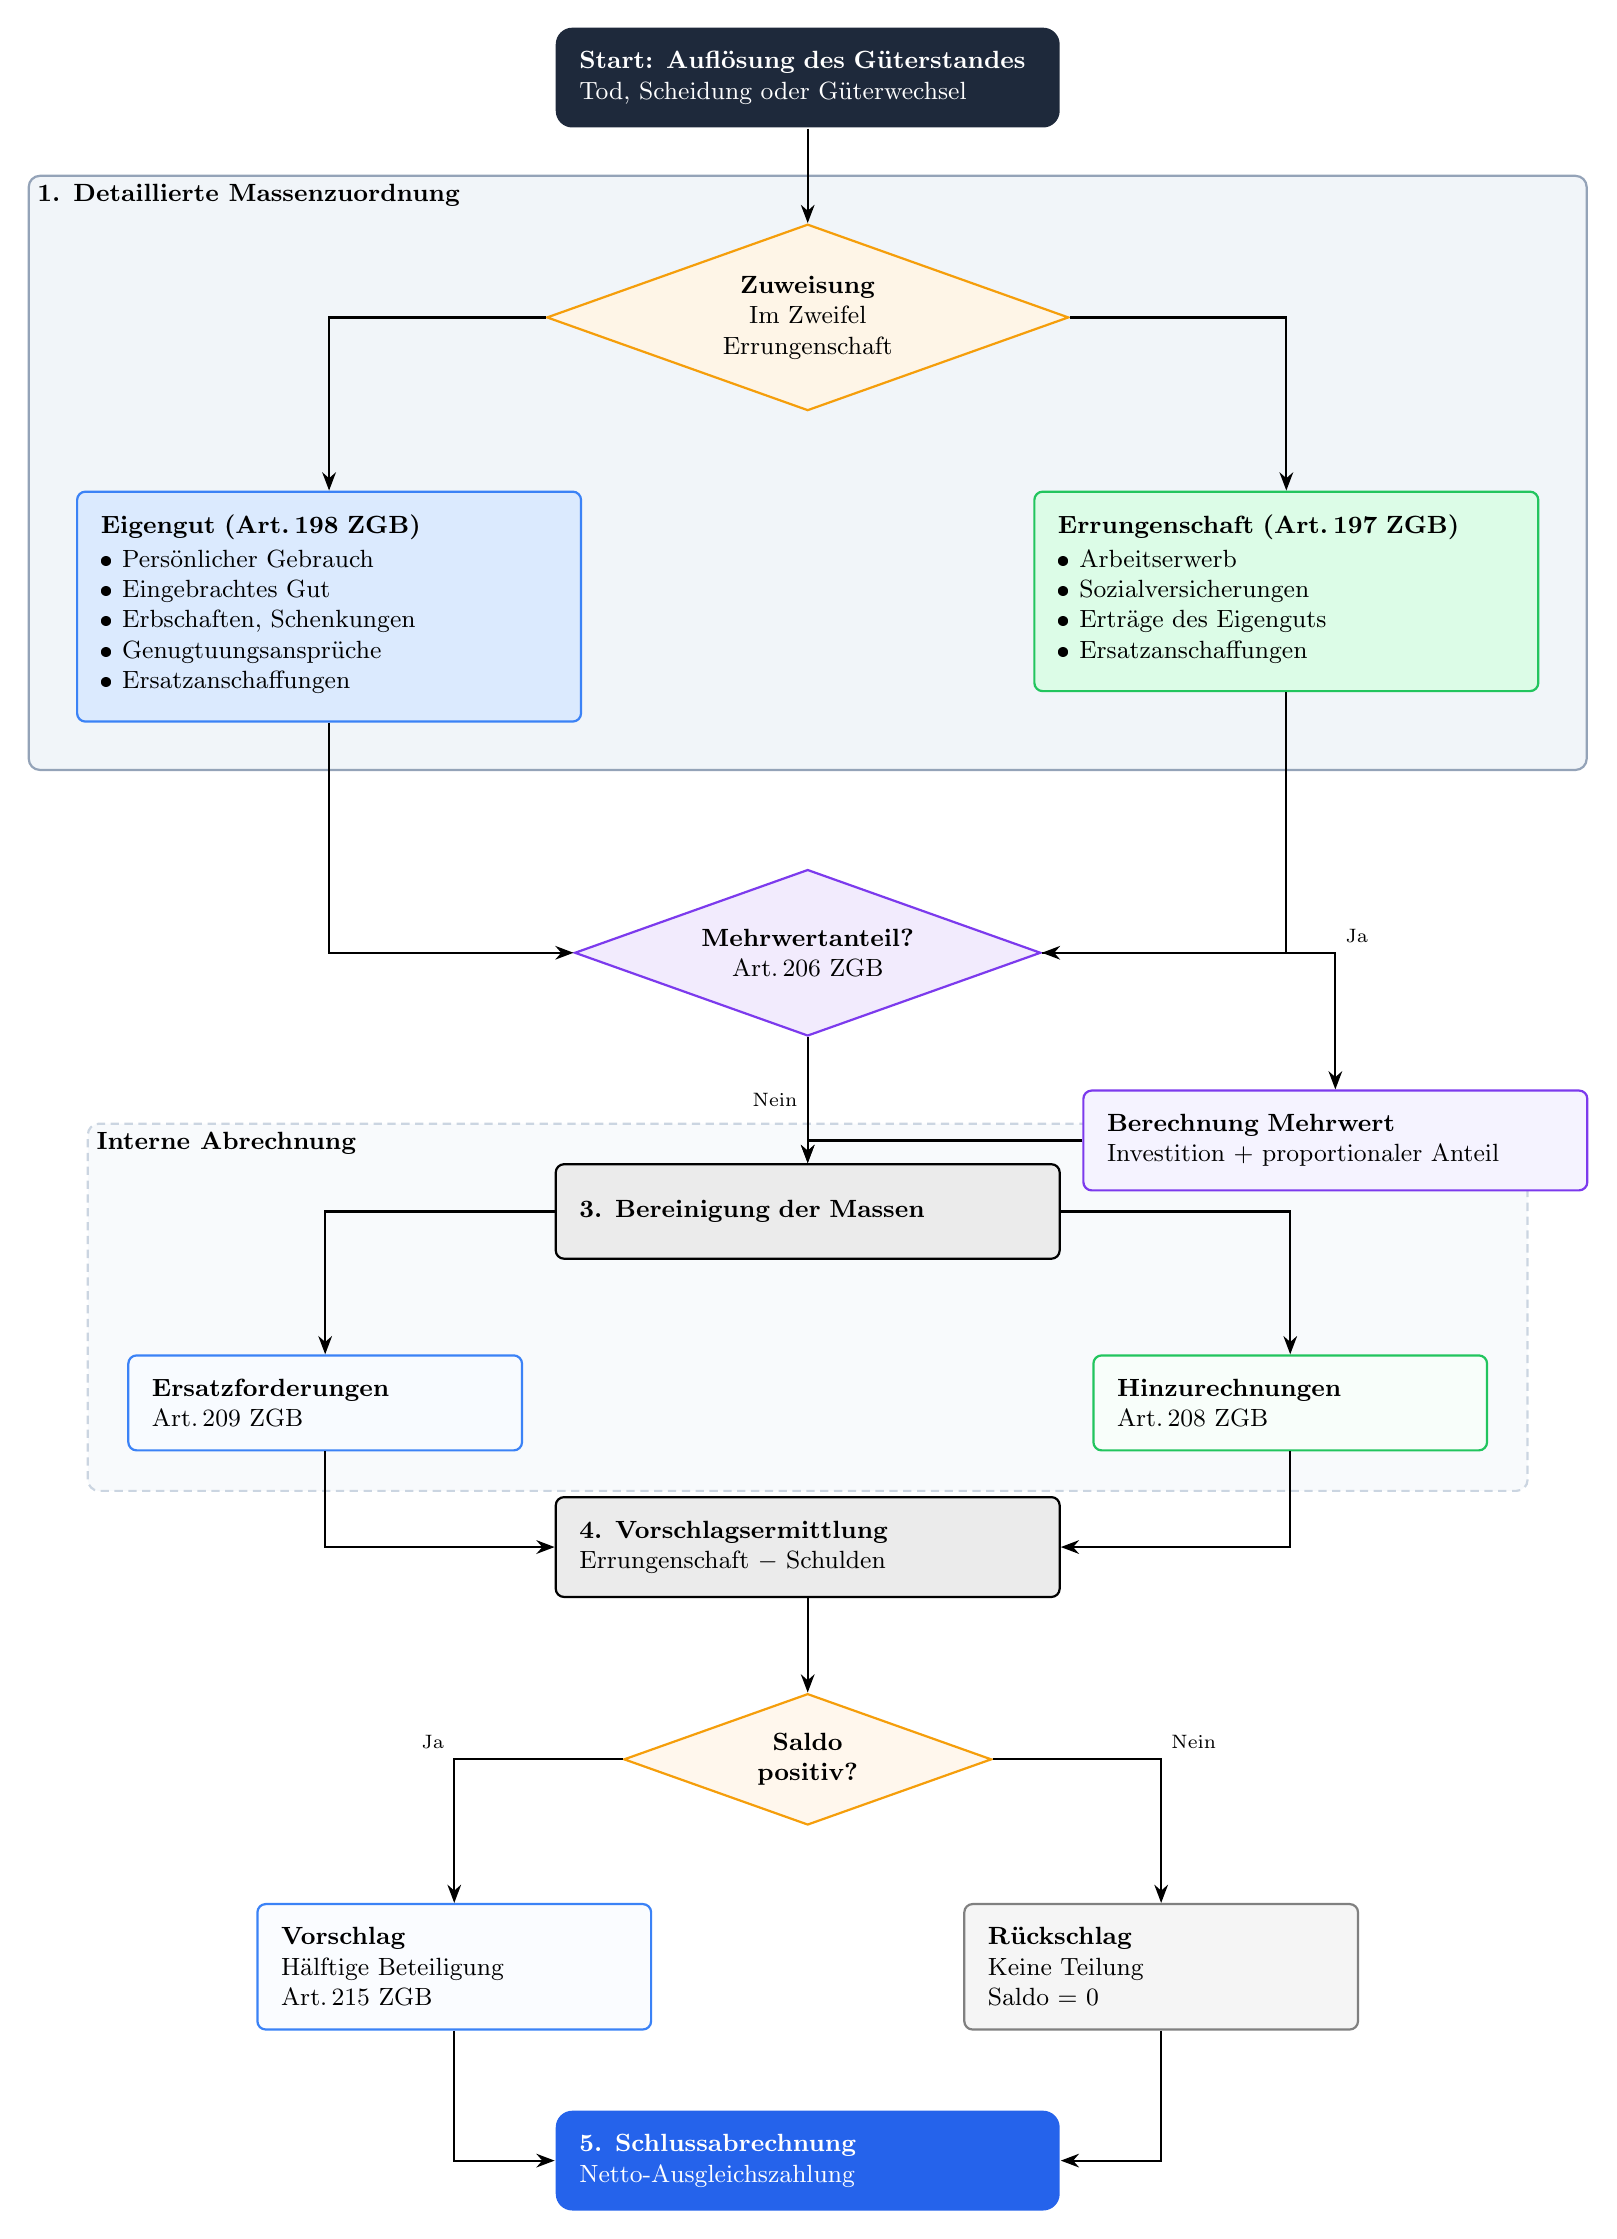
\begin{tikzpicture}[
    % ── Grundstile ──────────────────────────────────────
    node distance=10mm and 20mm,
    >=Stealth,
    every node/.style={font=\small},
    % Rechteck-Knoten
    block/.style={
        rectangle, rounded corners=3pt,
        draw=#1, fill=#1!8, thick,
        text width=58mm, minimum height=12mm,
        align=left, inner sep=3mm,
    },
    block/.default=black,
    % Rauten
    decision/.style={
        diamond, draw=#1, fill=#1!10, thick,
        align=center, inner sep=2mm,
        aspect=2.8,
    },
    decision/.default=clDecBorder,
    % Abgerundeter Start/Ende
    terminal/.style={
        rectangle, rounded corners=6pt,
        draw=none, fill=#1, thick,
        text width=58mm, minimum height=12mm,
        align=left, inner sep=3mm,
        font=\small\color{white},
    },
    % Pfeilstil
    arr/.style={->, thick, >=Stealth},
]

% ══════════════════════════════════════════════════════════
% Knoten
% ══════════════════════════════════════════════════════════

% ── Start ────────────────────────────────────────────────
\node[terminal=clStart] (start)
    {\textbf{Start: Auflösung des Güterstandes}\\
     Tod, Scheidung oder Güterwechsel};

% ── Schritt 1: Zuweisung ────────────────────────────────
\node[decision=clDecBorder, below=12mm of start] (step1)
    {\textbf{Zuweisung}\\
     Im Zweifel\\Errungenschaft};

% ── Eigengut / Errungenschaft nebeneinander ─────────────
\node[block=clEGborder, fill=clEG,
      below left=16mm and 12mm of step1] (eg)
    {\textbf{Eigengut (Art.\,198 ZGB)}\\[1pt]
     \tabcolsep=0pt
     \begin{tabular}{@{}l@{}}
     • Persönlicher Gebrauch\\
     • Eingebrachtes Gut\\
     • Erbschaften, Schenkungen\\
     • Genugtuungsansprüche\\
     • Ersatzanschaffungen
     \end{tabular}};

\node[block=clERborder, fill=clER,
      below right=16mm and 12mm of step1] (er)
    {\textbf{Errungenschaft (Art.\,197 ZGB)}\\[1pt]
     \tabcolsep=0pt
     \begin{tabular}{@{}l@{}}
     • Arbeitserwerb\\
     • Sozialversicherungen\\
     • Erträge des Eigenguts\\
     • Ersatzanschaffungen
     \end{tabular}};

% ── Schritt 2: Mehrwert ─────────────────────────────────
\node[decision=clMWborder,
      below=30mm of step1,
      yshift=-28mm] (step2)
    {\textbf{Mehrwertanteil?}\\Art.\,206 ZGB};

\node[block=clMWborder, fill=clMehrwert,
      below right=12mm and 20mm of step2] (mwcalc)
    {\textbf{Berechnung Mehrwert}\\
     Investition + proportionaler Anteil};

% ── Schritt 3: Bereinigung ──────────────────────────────
\node[block, below=16mm of step2] (step3)
    {\textbf{3. Bereinigung der Massen}};

\node[block=clEGborder, fill=clEG!20,
      below left=12mm and 4mm of step3,
      text width=44mm] (ersatz)
    {\textbf{Ersatzforderungen}\\Art.\,209 ZGB};

\node[block=clERborder, fill=clER!20,
      below right=12mm and 4mm of step3,
      text width=44mm] (hinzu)
    {\textbf{Hinzurechnungen}\\Art.\,208 ZGB};

% ── Schritt 4: Vorschlag ────────────────────────────────
\node[block, below=30mm of step3] (step4)
    {\textbf{4. Vorschlagsermittlung}\\
     Errungenschaft $-$ Schulden};

% ── Entscheidung positiv? ────────────────────────────────
\node[decision=clDecBorder, fill=clDecision,
      below=12mm of step4] (dec)
    {\textbf{Saldo}\\\textbf{positiv?}};

% ── Vorschlag / Rückschlag ──────────────────────────────
\node[block=clEGborder, fill=clEG!15,
      below left=14mm and 8mm of dec,
      text width=44mm] (vorschlag)
    {\textbf{Vorschlag}\\
     Hälftige Beteiligung\\Art.\,215 ZGB};

\node[block=gray, fill=gray!8,
      below right=14mm and 8mm of dec,
      text width=44mm] (rs)
    {\textbf{Rückschlag}\\
     Keine Teilung\\Saldo = 0};

% ── Schlussabrechnung ────────────────────────────────────
\node[terminal=clFinal,
      below=20mm of dec, yshift=-16mm] (final)
    {\textbf{5. Schlussabrechnung}\\
     Netto-Ausgleichszahlung};

% ══════════════════════════════════════════════════════════
% Pfeile
% ══════════════════════════════════════════════════════════

\draw[arr] (start)  -- (step1);
\draw[arr] (step1)  -| (eg);
\draw[arr] (step1)  -| (er);
\draw[arr] (eg.south)  |- (step2);
\draw[arr] (er.south)  |- (step2);

\draw[arr] (step2) -| node[above right]{\scriptsize Ja} (mwcalc);
\draw[arr] (step2) -- node[left]{\scriptsize Nein} (step3);
\draw[arr] (mwcalc.west) -| (step3);

\draw[arr] (step3) -| (ersatz);
\draw[arr] (step3) -| (hinzu);
\draw[arr] (ersatz.south) |- (step4);
\draw[arr] (hinzu.south)  |- (step4);

\draw[arr] (step4) -- (dec);
\draw[arr] (dec) -| node[above left]{\scriptsize Ja} (vorschlag);
\draw[arr] (dec) -| node[above right]{\scriptsize Nein} (rs);
\draw[arr] (vorschlag.south) |- (final);
\draw[arr] (rs.south)        |- (final);

% ══════════════════════════════════════════════════════════
% Hintergrund-Subgraphs (hinter den Knoten)
% ══════════════════════════════════════════════════════════
\begin{scope}[on background layer]
    % Massenzuordnung
    \node[fill=clSubgraphBG, draw=clSubgraphBorder, thick,
          rounded corners=4pt,
          fit=(step1)(eg)(er),
          inner sep=6mm,
          label={[anchor=north west, font=\small\bfseries]
                 north west:1. Detaillierte Massenzuordnung}] {};

    % Interne Abrechnung
    \node[fill=clKorrekturBG, draw=clKorrekturBorder,
          densely dashed, thick,
          rounded corners=4pt,
          fit=(step3)(ersatz)(hinzu),
          inner sep=5mm,
          label={[anchor=north west, font=\small\bfseries]
                 north west:Interne Abrechnung}] {};
\end{scope}

\end{tikzpicture}
\end{document}